\section{P2: RNN depth and time}

\subsection{Learning rate sweeps}
Figure~\ref{fig:p2lr} and Table~\ref{tab:p2} cover the 55 supplied RNN runs. The 1-layer plain tanh RNN reaches 4.033 at $\lr=0.003$; stacking four plain layers does not help (4.081 at $0.001$) and collapses to the unigram loss 6.875 at $0.002$ and $0.004$. The modern 4-layer RNN (pre-norm, depth residuals, SwiGLU MLPs) reaches 3.516 at $\lr=0.002$, half a nat better than either plain model, and is the only RNN family that is stable across the whole sweep. Among its ablations the differences are small at the best rate: gated residuals 3.496, gated norm 3.506, post-norm 3.512, gated output 3.513, final norm 3.521, no pre-norm 3.482 (its best, at $0.002$), no residual 3.581, RoPE on the recurrent input 3.566. The differences show up at higher rates: no pre-norm has non-finite gradients at $0.004$, post-norm climbs to 4.26 and 6.39 at $0.002$ and $0.004$ with its global activation RMS reaching 4000 (Figure~\ref{fig:p2rms}), and final norm, gated residual and gated output lose 0.1 to 0.15 nats at $2\times$ the centre. Pre-norm and depth residuals buy stability and rate headroom more than loss at the best rate, which matches P1.

\begin{figure}[h]\centering
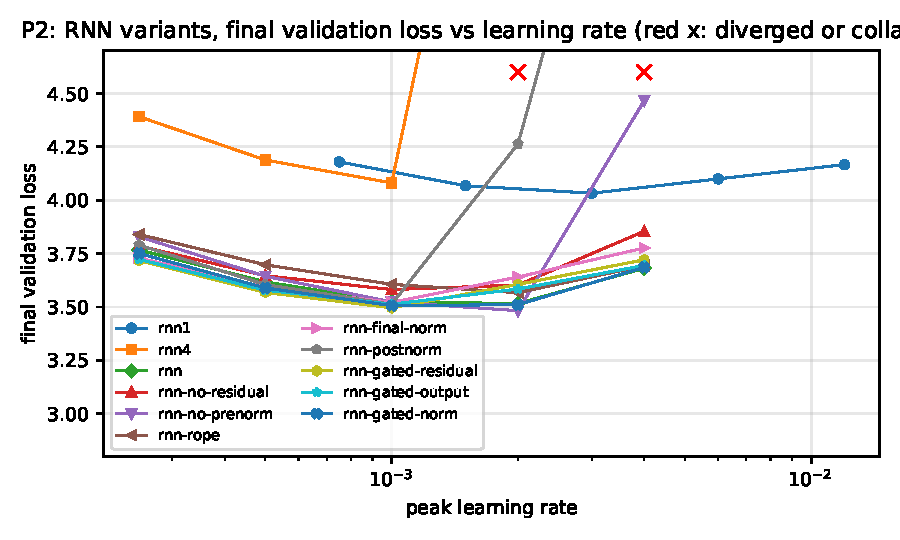
\includegraphics[width=.72\linewidth]{p2_lr_sweep.pdf}
\caption{P2 learning rate sweeps. Red crosses mark non-finite or collapsed runs.}
\label{fig:p2lr}
\end{figure}

\begin{table}[h]\centering\small
\caption{P2 final validation loss per rate (columns $0.25\times$ to $4\times$ each variant's centre; best in bold).}
\label{tab:p2}
\begin{tabular}{lrrrrrrr}\toprule
variant & best $\lr$ & $0.25\times$ & $0.5\times$ & $1\times$ & $2\times$ & $4\times$ & params (M)\\\midrule
rnn1 & 0.003 & 4.179 & 4.068 & \textbf{4.033} & 4.100 & 4.167 & 4.7 \\
rnn4 & 0.001 & 4.391 & 4.188 & \textbf{4.081} & 6.875 & 6.875 & 6.3 \\
rnn & 0.002 & 3.767 & 3.617 & 3.523 & \textbf{3.516} & 3.681 & 17.3 \\
rnn-no-residual & 0.001 & 3.785 & 3.646 & \textbf{3.581} & 3.602 & 3.855 & 17.3 \\
rnn-no-prenorm & 0.002 & 3.829 & 3.644 & 3.523 & \textbf{3.482} & 4.467 & 17.3 \\
rnn-rope & 0.002 & 3.839 & 3.697 & 3.606 & \textbf{3.566} & 3.694 & 17.3 \\
rnn-final-norm & 0.001 & 3.729 & 3.592 & \textbf{3.521} & 3.640 & 3.776 & 17.3 \\
rnn-postnorm & 0.001 & 3.789 & 3.605 & \textbf{3.512} & 4.263 & 6.389 & 17.3 \\
rnn-gated-residual & 0.001 & 3.717 & 3.568 & \textbf{3.496} & 3.605 & 3.721 & 19.4 \\
rnn-gated-output & 0.001 & 3.722 & 3.578 & \textbf{3.513} & 3.584 & 3.694 & 17.3 \\
rnn-gated-norm & 0.001 & 3.751 & 3.589 & \textbf{3.506} & 3.511 & 3.685 & 19.4 \\
\bottomrule\end{tabular}

\end{table}

\begin{figure}[h]\centering
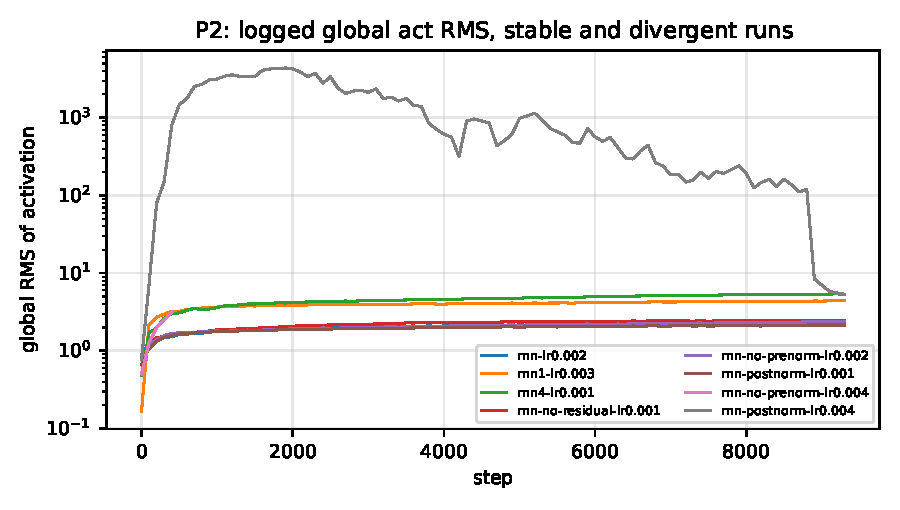
\includegraphics[width=.49\linewidth]{p2_rms_act.pdf}
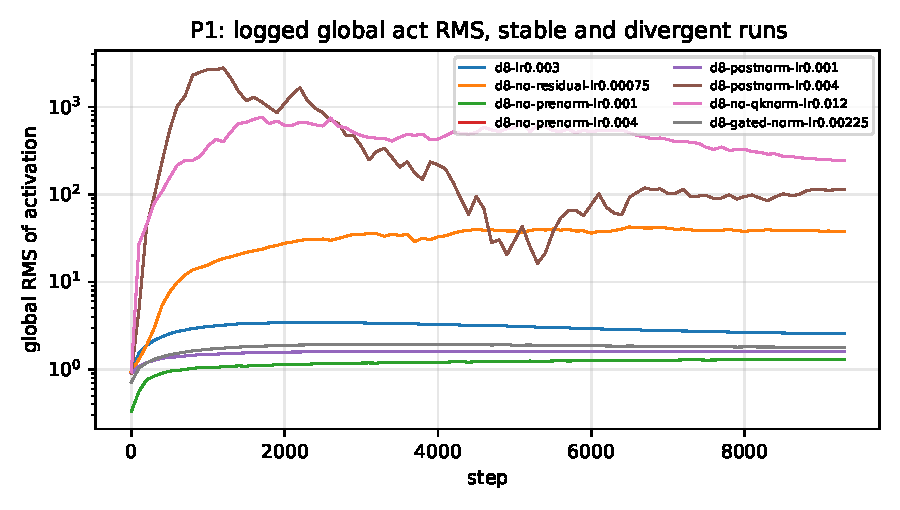
\includegraphics[width=.49\linewidth]{p1_rms_act.pdf}
\caption{Logged global activation RMS during training for stable and unstable RNN (left) and transformer (right) runs.}
\label{fig:p2rms}
\end{figure}

\subsection{Hidden state gradients, RMS and saturation}
Figure~\ref{fig:p2time} shows the last recurrent layer of the three main models on the final checkpoints. All three keep the hidden state RMS between 0.78 and 0.9, and 35\% (1 layer) to 55\% (4 layers) of the tanh units are saturated beyond 0.95 at every step. Under the full loss the gradient reaching $h_t$ is flat over time, because every position has its own target. Under the last-token loss the picture is the classic one: the gradient falls by about 32 orders of magnitude across the 1024 steps for the 1-layer RNN, and the plain 4-layer and modern RNNs underflow to zero after 250 and 90 steps respectively. The modern RNN has the shortest temporal gradient reach of the three because its upper layers are smooth in time (cosine between $h_t$ and $h_{t-64}$ is 0.93 in layer 4 versus 0.15 in the 1-layer model, Figure~\ref{fig:p2layers}): information flows forward along the depth residual, not back along time. The plain 4-layer model has intermediate smoothness (0.12 in layer 1 to 0.48 in layer 4) and shows the depth problem instead: its layer 1 hidden state gradient under the full loss is 3 times smaller than its layer 4 gradient at init and the stream gradient drops by 10 across the stack (Figure~\ref{fig:p2depth}).

\begin{figure}[h]\centering
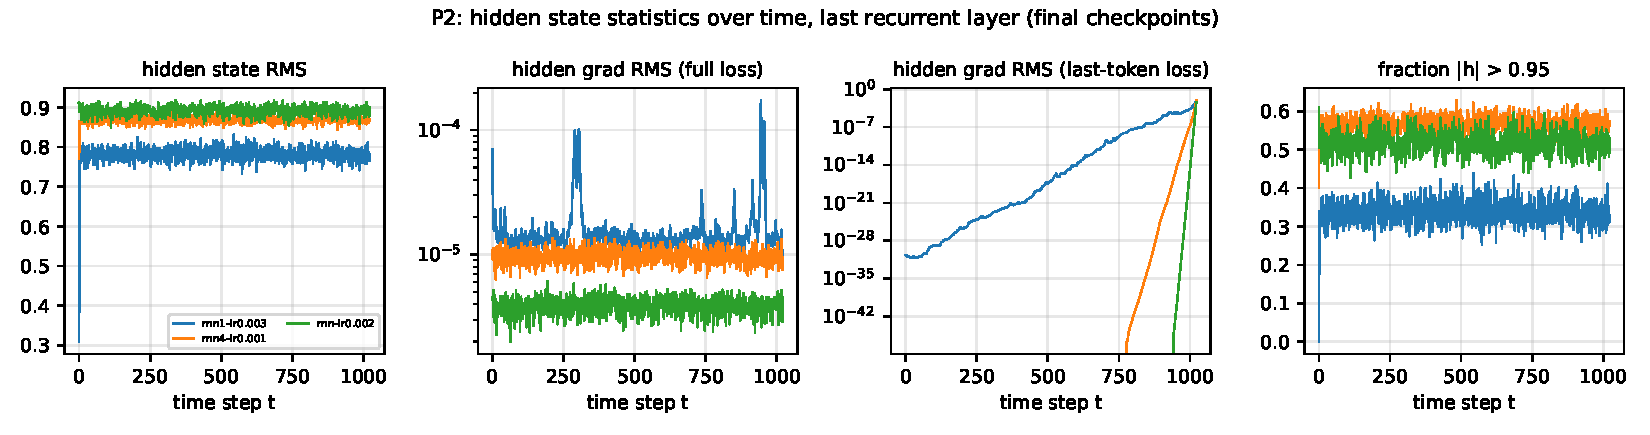
\includegraphics[width=\linewidth]{p2_temporal_plain_vs_modern.pdf}
\caption{Last recurrent layer over time for the 1-layer, plain 4-layer and modern RNNs (final checkpoints, 8 sequences).}
\label{fig:p2time}
\end{figure}

\begin{figure}[h]\centering
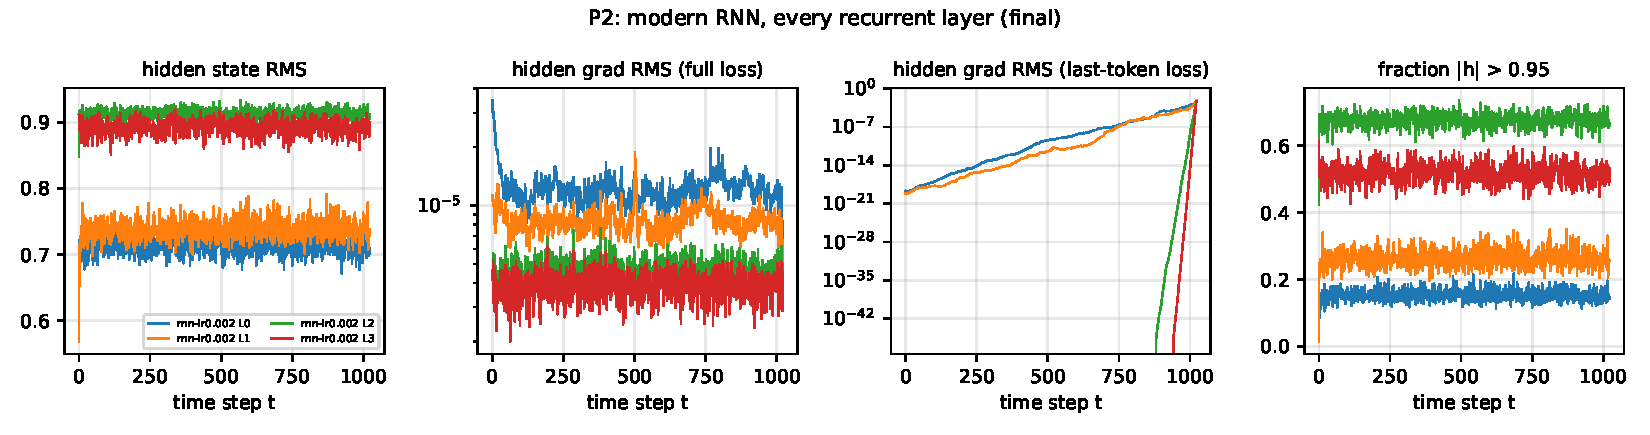
\includegraphics[width=\linewidth]{p2_temporal_rnn_layers.pdf}
\caption{Modern RNN: every recurrent layer over time (final checkpoint). Lower layers change fast, upper layers hold an almost constant state.}
\label{fig:p2layers}
\end{figure}

\subsection{Depth}
Figure~\ref{fig:p2depth} gives the depth profiles. The modern RNN's stream grows from 0.11 to 1.7 over 8 branches, with the cosine between consecutive stream states between 0.75 and 0.97, so, as in the transformer, each branch is a correction to a shared stream. Without depth residuals the stream has cosine 0 between consecutive states and the branch to input ratio alternates between 0.3 and 5: the recurrent branches contract and the MLPs expand. The no-residual, no-prenorm and post-norm ablations also have the largest upper layer temporal cosines (0.998 and 0.999 in layers 3 and 4 for no-prenorm and RoPE), that is, their upper layers have essentially frozen their hidden state and act as feedforward layers. Figure~\ref{fig:p2stages} shows that, unlike the transformer, the modern RNN's depth profile is already in its final shape at initialisation; training changes the embedding gradient by 10 and little else.

\begin{figure}[h]\centering
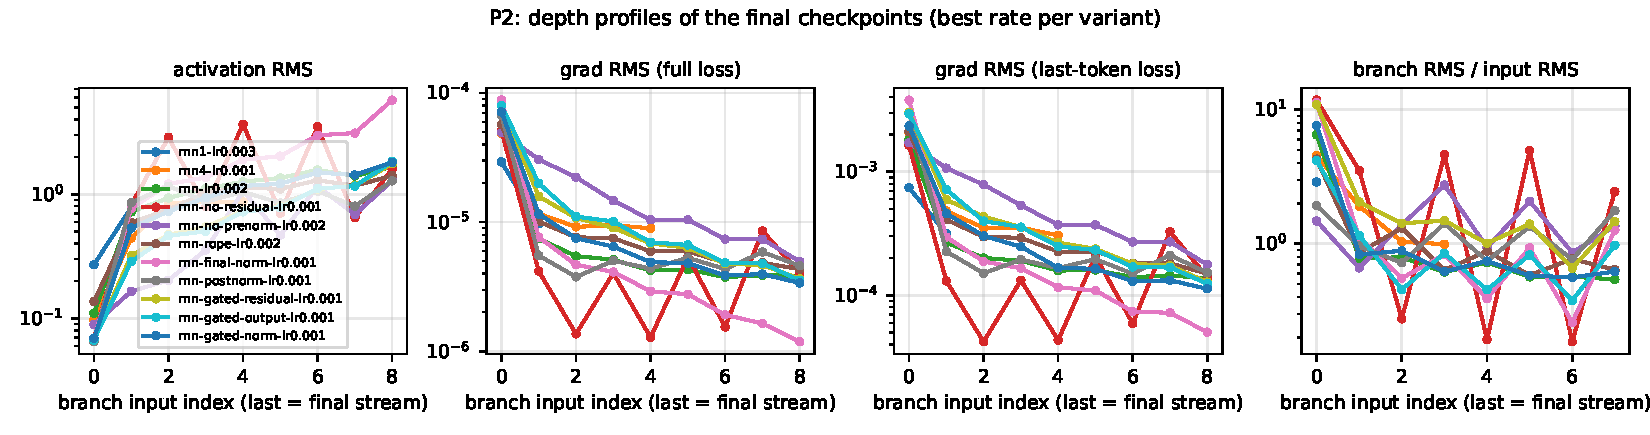
\includegraphics[width=\linewidth]{p2_depth_final.pdf}
\caption{P2 depth profiles (final checkpoints, best rate per variant). Even indices are recurrent branch inputs, odd are MLP inputs, index 8 is the final stream.}
\label{fig:p2depth}
\end{figure}

\begin{figure}[h]\centering
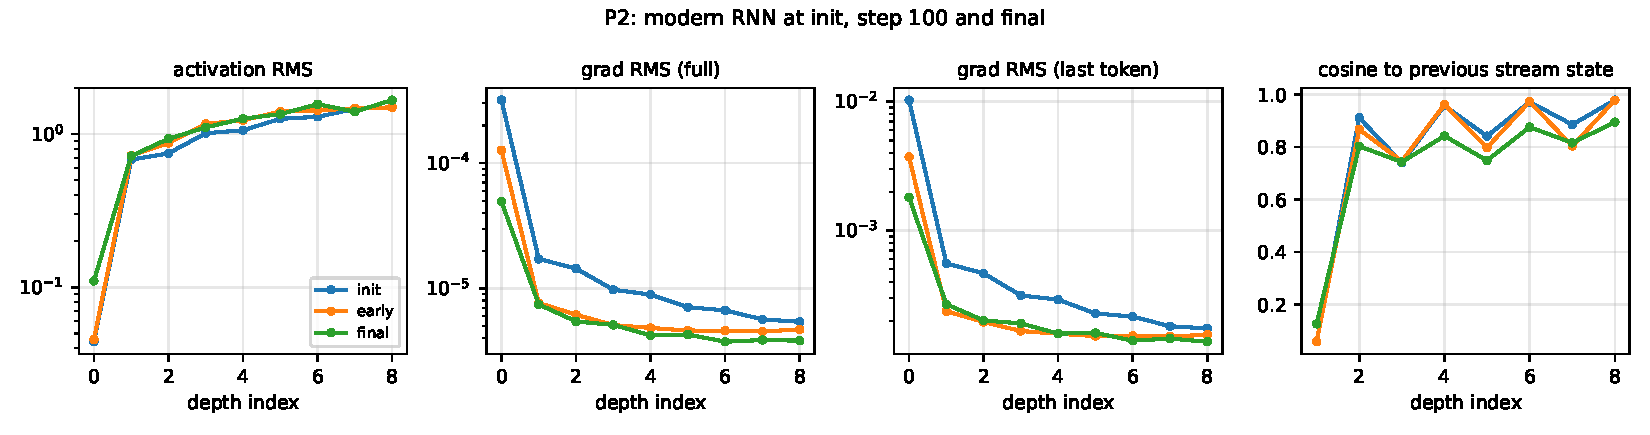
\includegraphics[width=\linewidth]{p2_rnn_stages.pdf}
\caption{Modern RNN at initialisation, step 100 and the final checkpoint.}
\label{fig:p2stages}
\end{figure}

\subsection{Context use and the first token}
Table~\ref{tab:p2ctx} gives the RNN context tests. With the first token restored all RNNs lose about 1.2 to 1.9 nats with one recent token, 0.2 to 0.5 with four and nothing measurable beyond 64, in line with the gradient reach above. Without the first token the plain RNNs are unaffected beyond 16 tokens, but the modern RNN loses 40 to 56 nats at every context length, including 512 tokens. Its upper layers hold a near constant state, that state is set by the first token (which the model always sees at position 0 in training), and starting the recurrence from $h_0$ on a mid-document token drives it into a regime from which it never recovers. The RoPE variant behaves the same way, with a 700 nat increase at one token. This is the recurrent analogue of the no-RoPE transformer's dependence on the sink token, and it is why the handout asks for the first token to be restored and the state to be reset correctly.

\begin{table}[h]\centering\small
\caption{Increase of the last token loss (nats) when only $k$ recent tokens are kept; recurrent state reset; final checkpoints; 64 sequences.}
\label{tab:p2ctx}
\begin{tabular}{llrrrrrr}\toprule
model & first token & $k=1$ & 2 & 4 & 16 & 64 & 512\\\midrule
rnn1 & dropped & 1.57 & 0.74 & 0.23 & 0.01 & 0.01 & 0.00\\
rnn1 & restored & 1.22 & 0.67 & 0.28 & 0.03 & 0.00 & 0.00\\
rnn4 & dropped & 3.48 & 2.75 & 1.06 & 0.04 & 0.01 & 0.00\\
rnn4 & restored & 1.27 & 0.61 & 0.26 & 0.04 & 0.00 & 0.00\\
rnn (modern) & dropped & 42.3 & 50.5 & 54.9 & 56.1 & 49.1 & 54.6\\
rnn (modern) & restored & 1.91 & 1.07 & 0.50 & 0.16 & 0.00 & 0.00\\
rnn-gated-residual & dropped & 2.27 & 1.07 & 0.43 & 0.11 & 0.00 & 0.00\\
rnn-gated-residual & restored & 1.86 & 1.03 & 0.44 & 0.15 & 0.03 & 0.00\\
d8 transformer & dropped & 6.56 & 4.78 & 4.07 & 1.73 & 0.48 & 0.00\\
d8 transformer & restored & 6.42 & 2.98 & 1.56 & 0.47 & 0.19 & 0.00\\
d8 no RoPE & dropped & 4.68 & 4.55 & 4.44 & 4.49 & 4.52 & 4.61\\
d8 no RoPE & restored & 2.08 & 1.26 & 0.65 & 0.21 & 0.09 & 0.00\\
\bottomrule\end{tabular}
\end{table}
